\documentclass[a4paper,14pt]{article}

\usepackage{cmap}                       % поиск в PDF
\usepackage{mathtext}                   % русские буквы в фоhмулах
\usepackage[T2A]{fontenc}               % кодировка
\usepackage[utf8]{inputenc}             % кодировка исходного текста
\usepackage[english,russian]{babel}     % локализация и переносы

\usepackage{amsmath,amsfonts,amssymb,amsthm,mathtools}
\usepackage{icomma}

\newcommand*{\hm}[1]{#1\nobreak\discretionary{}
{\hbox{$\mathsurround=0pt #1$}}{}}

\mathtoolsset{showonlyrefs=true}

\usepackage{geometry}
\geometry{top=15mm}
\geometry{bottom=15mm}
\geometry{left=15mm}
\geometry{right=15mm}

\everymath{\displaystyle}

% Колонтитулы
\usepackage{fancyhdr}
\pagestyle{fancy}
\fancyhf{}
\rhead{Пути}
\lhead{2020}

\begin{document}
\section*{Пути}
\subsection*{Биномиальный коэффициент}
\textbf{Задача:} Двигаясь только вправо или только вверх,
найти количество путей из $\left(0, 0\right) в \left(n, m\right)$.
Нетрудно убедиться, что таких путей $\binom{n + m}{m}$.
Найдем для них производящую функцию:
\begin{align*}
	A(x, y) =\sum_{n,m=0}^{\infty}\binom{n + m}{m}x^ny^m = 
\sum_{k = 0}^{\infty}\left( \sum_{m+n=k}^{\infty} \binom{n + m}{m}x^ny^m \right) =
\sum_{k=0}^{\infty} \left(x + y\right)^k = \dfrac{1}{1 - x - y} 
.\end{align*}
\begin{figure}[htpb]
	\centering
	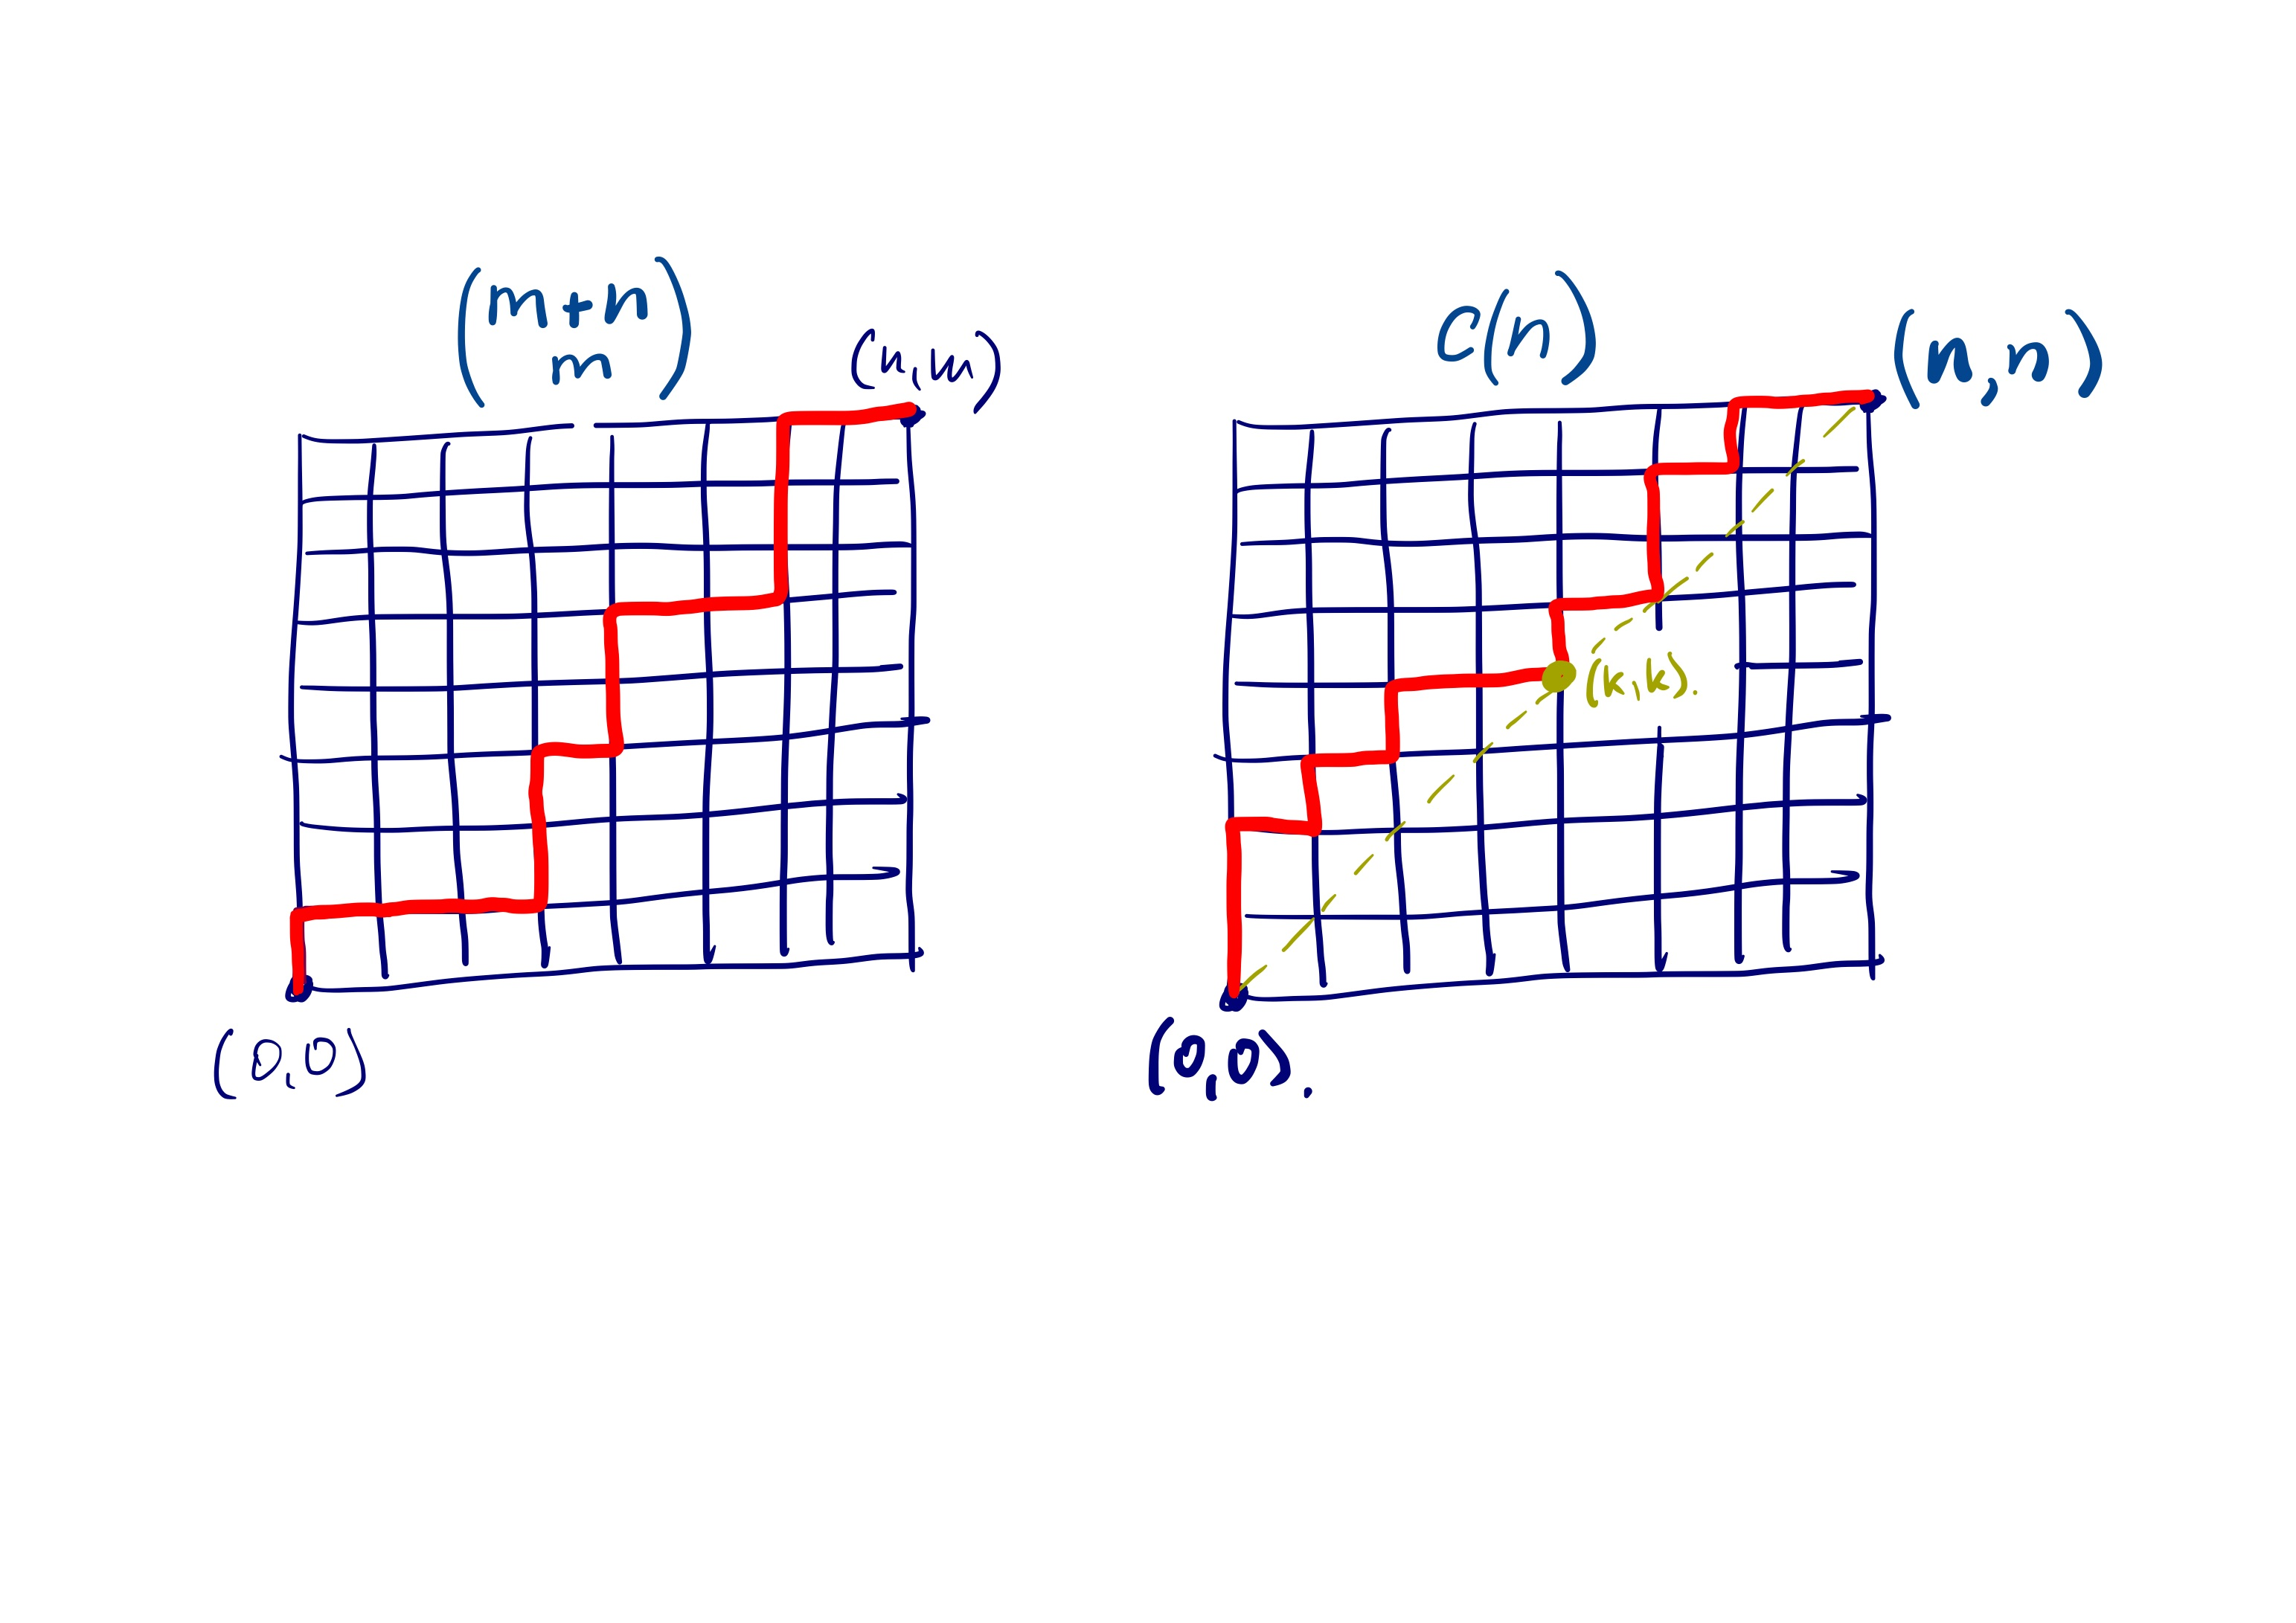
\includegraphics[width=0.8\textwidth]{images/path1}
	\caption{Слева: пути вверх-вправо из $(0, 0)$ в $(n,m)$, Справа:
	пути вверх-вправо выше диагонали}
	\label{fig:}
\end{figure}
\subsection*{Числа Каталана}
Рассмотрим количество путей из $\left( 0, 0 \right) $ в $\left( n, n \right) $,
пролегающих выше прямой $y = x$. \\
Пусть $C(n)$ – искомое число путей. Тогда один из возможных способов дойти до
$\left(n, n\right) $ через точку $\left( k, k \right)$, где $k  \in \left[0, n\right)$ – это
все пути (их $C(k) $ штук) из $\left( 0, 0 \right) $ в $\left( k, k \right) $
умножить на все пути из $\left( k, k \right) $ в $\left( n, n \right) $, где их
$C(n - k - 1) $ штук. Тогда по всем имеющимся $k$ получаем реккурентное выражение для 
чисел Каталана:
\begin{align*}
	C(n) = \sum_{k=0}^{n - 1} C(k) \cdot  C(n - k - 1)
.\end{align*}
\begin{figure}[!htpb]
	\centering
	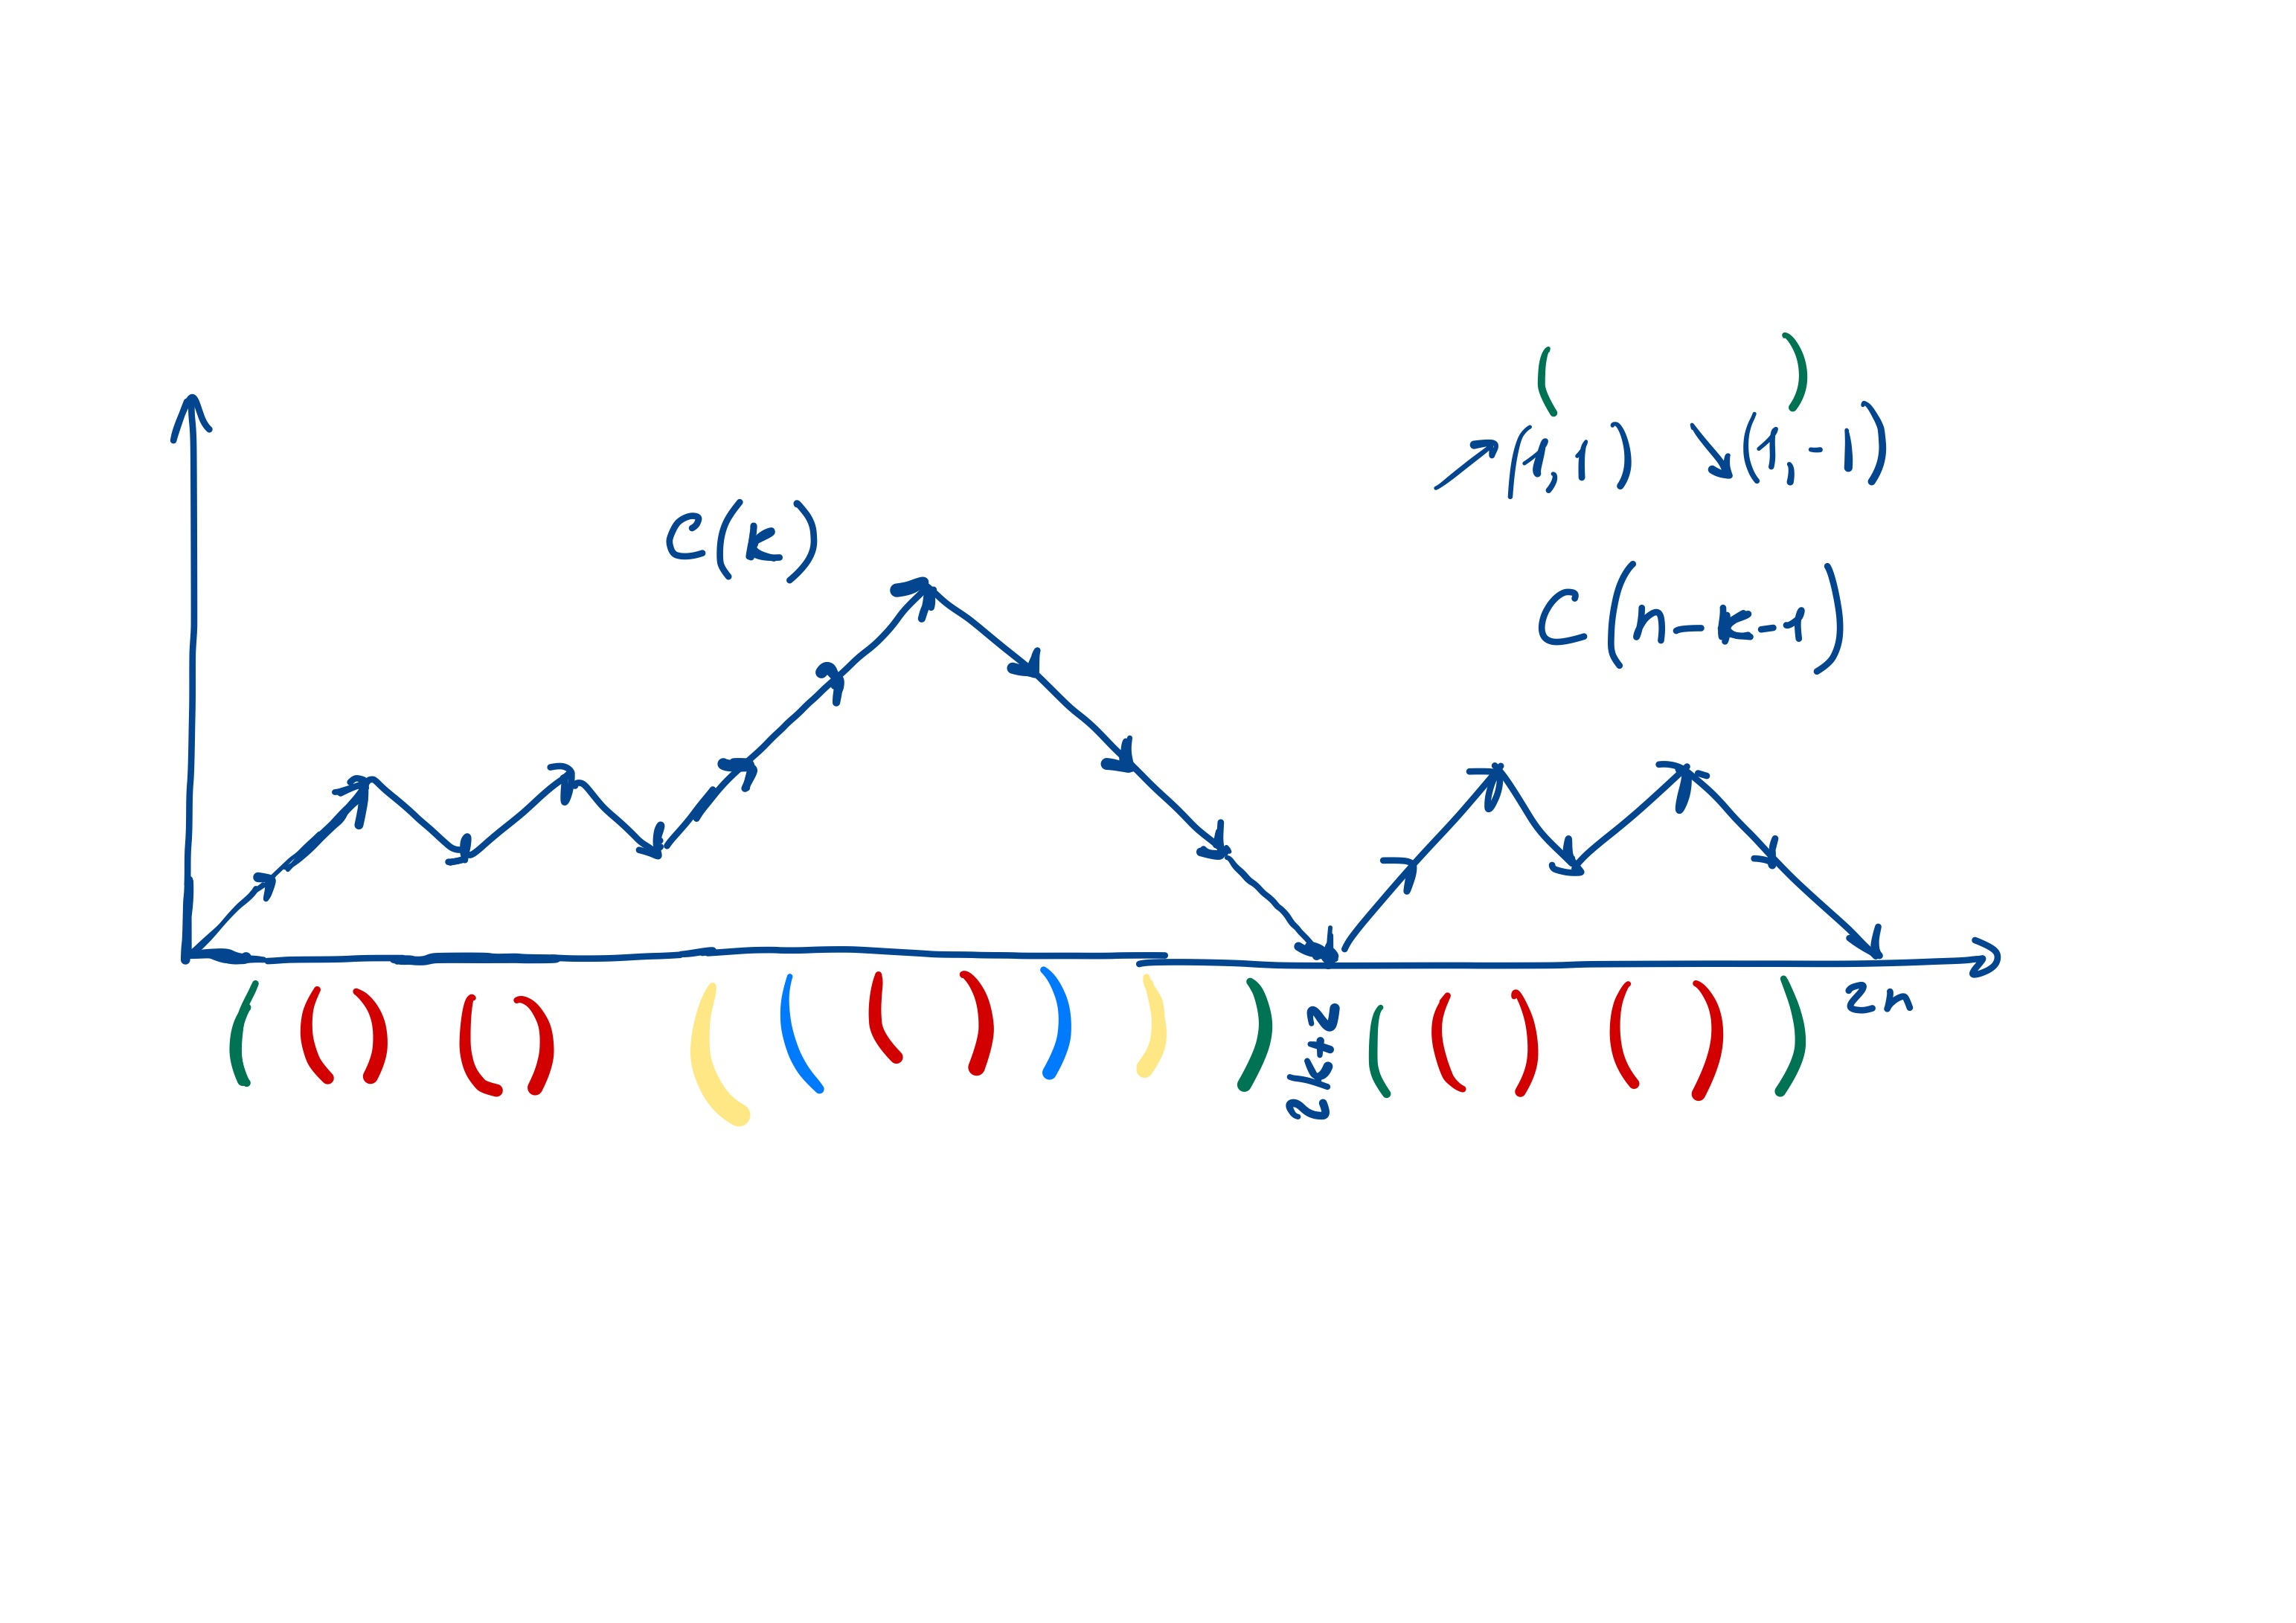
\includegraphics[width=0.8\textwidth]{images/dyck}
	\caption{Путь Дика и правильная скобочная последовательность}
	\label{fig:dyck}
\end{figure}
Найдем для C(n) производящую функцию:
\begin{align*}
	K(q) &= \sum_{n=0}^{\infty} C(n)q^n = 1 + q + 2q^2 + 5q^3 + 14q^4 + \ldots = \ ? \\
	K^2(q) &= \sum_{n=0}^{\infty}\left( \sum_{k=0}^{n - 1}C(k) \cdot C(n - k - 1) \right) q^n \\
	qK^2(q) & = \sum_{n=0}^{\infty}\left( \sum_{k=0}^{n - 1}C(k) \cdot C(n - k - 1) \right) q^{n + 1} =
	\sum_{n=1}^{\infty}\left( \sum_{k=0}^{n - 1}C(k) \cdot C(n - k - 1) \right) q^n \\
	qK^2(q) &= \sum_{n=1}^{\infty} C(n)q^n = K(q) - 1
.\end{align*}
Получив уравнение $qK^2(q) = K(q) - 1$, решим его для $K(q)$:
\[
	K(q) = \frac{1 - \sqrt{1 - 4q}}{2} \text{ – производящая функция для чисел Каталана.} 
\] 
\end{document}
